\section*{Conclusion}\addcontentsline{toc}{section}{Conclusion}
Maintenant que la conception de \emph{BedBihan} a été effectuée, nous pouvons passer au développement réel du projet. Le code généré automatiquement par Visual Studio 2013 --- le logiciel avec lequel nous avons réalisé notre diagramme de classe --- nous servira de base pour l'implémentation de toutes les fonctionnalités du jeu.


\newpage
\appendix
\section*{Annexe : diagramme de classes complet}\addcontentsline{toc}{section}{Annexe : diagramme de classes complet}
Ce diagramme illustre la structure globale de \emph{BedBihan}. Toutefois, pour une meilleure lisibilité des détails de ce diagramme, la consultation du fichier PNG joint avec ce rapport est vivement recommandée.
\begin{figure}[hb]
		\begin{center}
			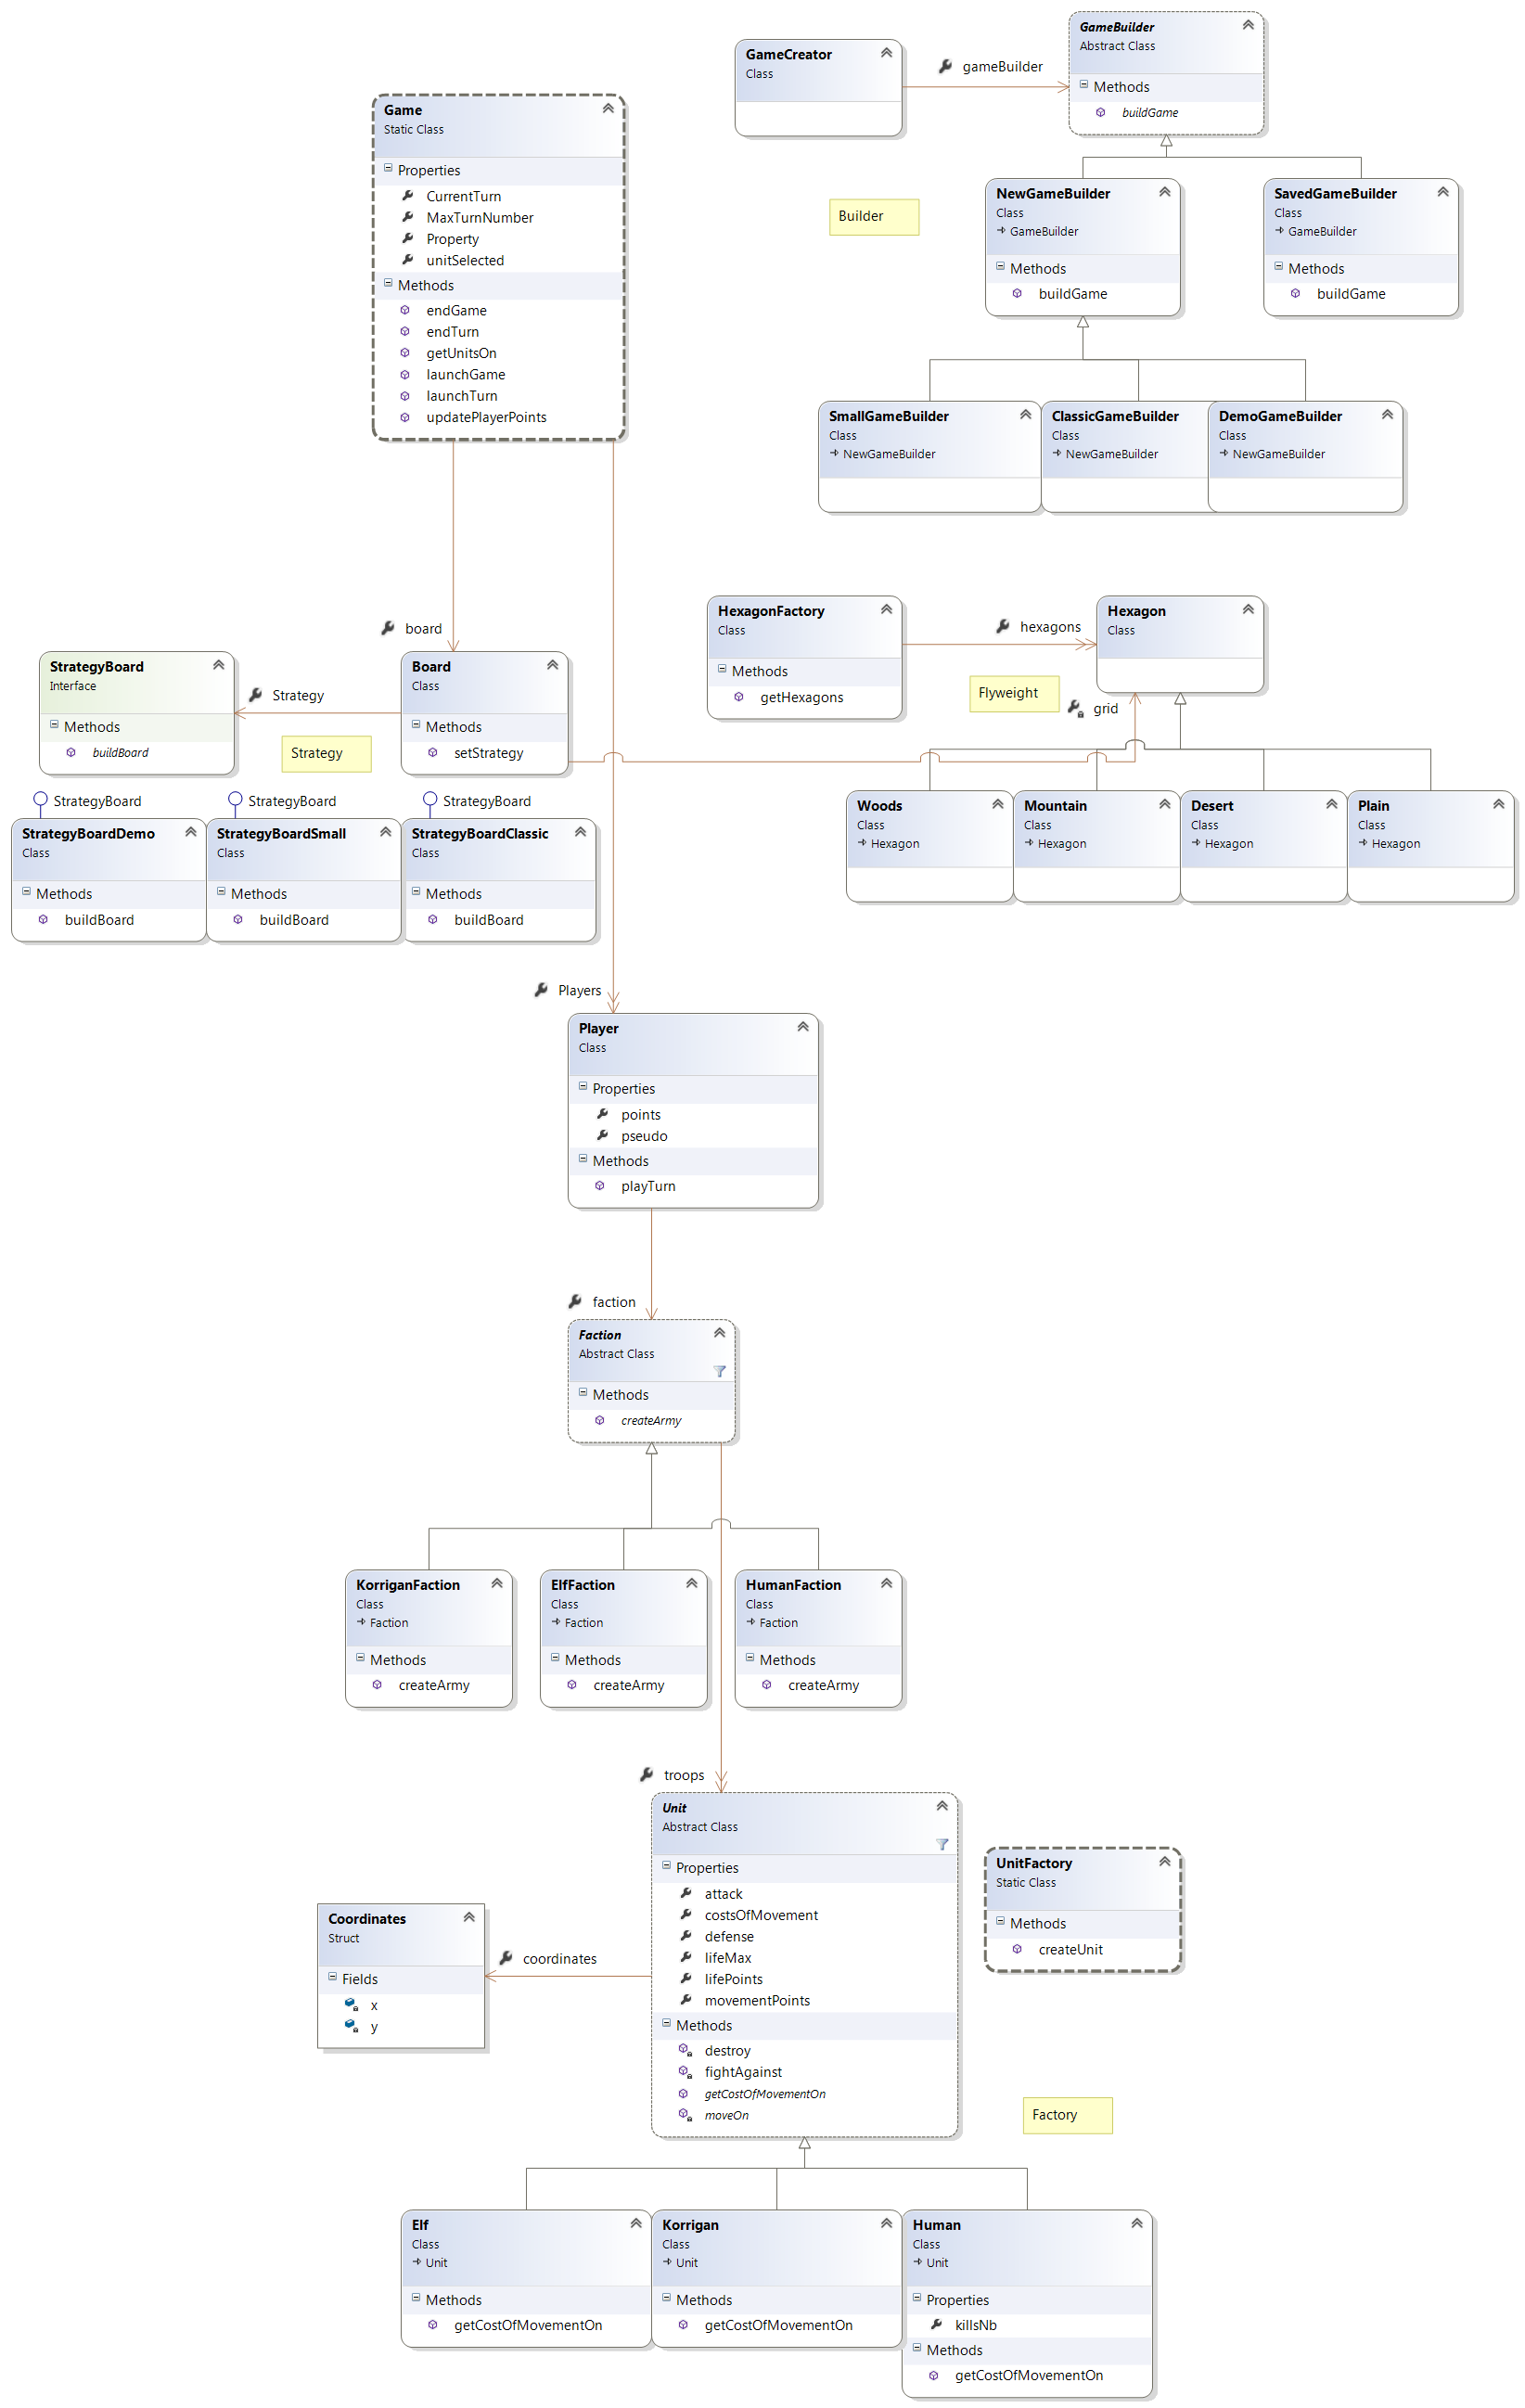
\includegraphics[width=0.7\textwidth]{figure/entire_class_diagram_report.png}
		\end{center}
		
		\label{fig:class_global}
	\end{figure}